
\documentclass[11pt]{article}

\usepackage[utf8]{inputenc}
\usepackage[T1]{fontenc}
\usepackage{lmodern}
\usepackage{geometry}
\geometry{margin=1in}

\usepackage{amsmath, amssymb, amsfonts, mathtools}
\usepackage{booktabs}
\usepackage{tabularx}
\usepackage{microtype}
\usepackage{hyperref}
\usepackage{pgfplots}
\pgfplotsset{compat=1.18}

\setlength{\parindent}{0pt}
\setlength{\parskip}{0.6em}

\title{Business Outcomes and Psychological Difference:\\
A Mathematical Analysis of Agreeableness and Income Disparity}
\author{}
\date{}

\begin{document}
\maketitle

\section{Psychological Traits as Economic Variables}

In labor economics and organizational psychology, personality traits are modeled as
\emph{latent individual differences} that systematically affect market outcomes.
Let
\[
A \in \mathbb{R}
\]
denote an individual's standardized agreeableness score (mean $0$, variance $1$),
as measured by Big Five psychometrics.

Empirically, agreeableness reflects tendencies toward cooperation, compliance,
conflict avoidance, and prosocial behavior. These traits interact directly with
negotiation behavior, promotion dynamics, and compensation structures in firms.

\section{Income as a Function of Psychological Traits}

Let annual income be modeled as
\[
Y = f(A, X) + \varepsilon,
\]
where:
\begin{itemize}
  \item $A$ = agreeableness
  \item $X$ = vector of controls (education, experience, occupation, cognitive ability)
  \item $\varepsilon$ = idiosyncratic noise
\end{itemize}

A first\-order approximation yields a linear earnings equation:
\begin{equation}
\log Y = \beta_0 + \beta_A A + \beta_X X + \varepsilon.
\end{equation}

\section{Magnitude of the Income Penalty}

Empirical estimates place $\beta_A$ in the range
\[
\beta_A \approx -0.05 \;\; \text{to} \;\; -0.10,
\]
implying that a one\-standard\-deviation increase in agreeableness corresponds to
a \emph{5--10\% decrease in income}.

Thus, comparing two individuals identical in all respects except agreeableness:
\[
\frac{Y_{\text{low }A}}{Y_{\text{high }A}}
\approx e^{-\beta_A \Delta A}.
\]

For $\Delta A = 2$ (one SD below vs one SD above the mean),
\[
\frac{Y_{\text{low }A}}{Y_{\text{high }A}} \approx 1.10 \text{--} 1.22.
\]

\section{Mechanism: Business Interaction Model}

This disparity arises from repeated strategic interactions.
Let wage growth be modeled as:
\[
\Delta Y_t = g(N_t, C_t, A),
\]
where:
\begin{itemize}
  \item $N_t$ = negotiation frequency
  \item $C_t$ = conflict tolerance
  \item $A$ = agreeableness
\end{itemize}

Empirically one expects
\[
\frac{\partial N_t}{\partial A} < 0,
\quad
\frac{\partial C_t}{\partial A} < 0,
\]
which suppresses cumulative wage growth over time.

\section{Income Distribution Conditional on Agreeableness}

Let income conditional on agreeableness be log\-normally distributed:
\[
Y \mid A \sim \text{LogNormal}(\mu(A), \sigma^2),
\quad
\mu(A) = \mu_0 + \beta_A A.
\]

Then expected income is:
\[
\mathbb{E}[Y \mid A] = \exp\!\left(\mu_0 + \beta_A A + \frac{\sigma^2}{2}\right),
\]
which is strictly decreasing in $A$ when $\beta_A < 0$.

\section{Graphical Representation}

\begin{center}
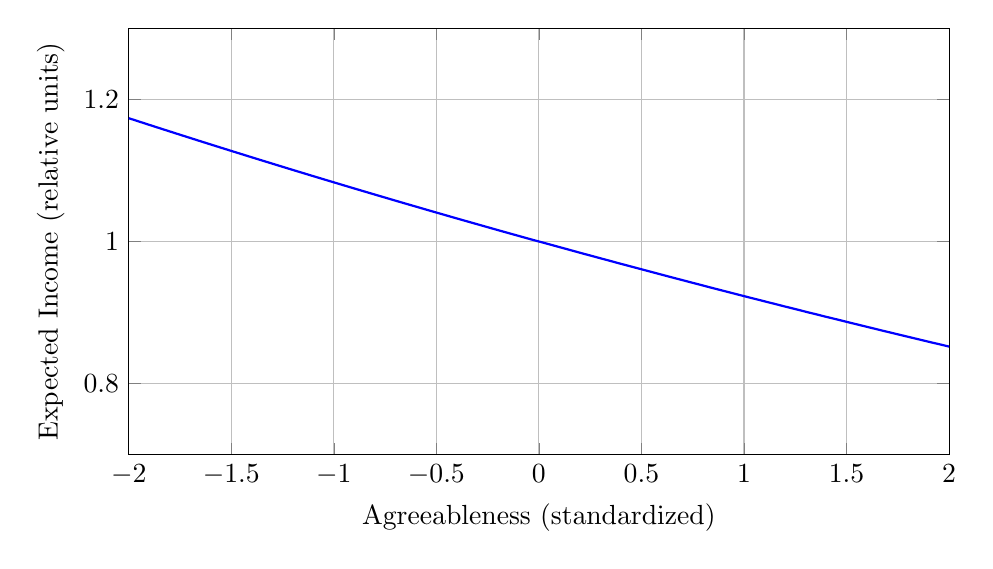
\begin{tikzpicture}
\begin{axis}[
  width=12cm,
  height=7cm,
  xlabel={Agreeableness (standardized)},
  ylabel={Expected Income (relative units)},
  xmin=-2, xmax=2,
  ymin=0.7, ymax=1.3,
  domain=-2:2,
  samples=100,
  grid=both,
]
\addplot[thick, blue] {exp(-0.08*x)};
\end{axis}
\end{tikzpicture}
\end{center}

This curve represents:
\[
\mathbb{E}[Y \mid A] \propto e^{\beta_A A},
\quad \beta_A = -0.08.
\]

\section{Interpretation for Business Systems}

From a systems perspective:
\begin{itemize}
  \item Firms reward \emph{assertive surplus extraction}.
  \item Agreeableness increases cooperation but reduces bargaining leverage.
  \item Markets price outcomes, not intentions.
\end{itemize}

Hence, agreeableness acts as a \emph{negative return personality factor}
in competitive compensation environments.

\section{Conclusion}

Mathematically and empirically:
\[
\boxed{\; \frac{\partial \mathbb{E}[Y]}{\partial A} < 0 \;}
\]

Agreeableness improves social harmony but is associated with a measurable income penalty in
business environments governed by negotiation, competition, and asymmetric power.

\end{document}
